%----------------------------------------------------------------------------------------
%	PACKAGES AND OTHER DOCUMENT CONFIGURATIONS
%----------------------------------------------------------------------------------------

\documentclass[a4paper,11pt]{article} % Font and paper size

%----------------------------------------------------------------------------------------
%	PACKAGES AND OTHER DOCUMENT CONFIGURATIONS
%----------------------------------------------------------------------------------------

\usepackage[utf8]{inputenc} % Required for inputting international characters
\usepackage[T1]{fontenc} % Output font encoding for international characters
\usepackage[italian]{babel} % Italian dictionary


\usepackage[table]{xcolor} % Required for custom colors
\usepackage{gensymb}
\usepackage{amsmath}
\usepackage{bm}
\usepackage{tikz}
\usepackage{hhline}
\usepackage{listings}
\usepackage{enumitem}

%\usepackage[margin=2cm, includefoot]{geometry} % Modify margins
\usepackage{fancyhdr}
\usepackage{rotating}
\usepackage[hidelinks]{hyperref} % Hyperlinks

\usepackage[none]{hyphenat}% Non spezza le parole nelle tabelle
\usepackage{array}

\usepackage{graphicx} % Required for figures
\usepackage{float}
\usepackage{wrapfig}
\usepackage{caption}
\usepackage{subcaption}

%pagestyle
\pagestyle{fancy}
\fancyhead{}
\fancyfoot{}
\fancyfoot[R]{\thepage}
\renewcommand{\headrulewidth}{0pt}



\usepackage{xfrac}
\usepackage{amssymb}

\usepackage{multicol}
\usepackage{multirow}

\usepackage[toc, page]{appendix}
\usepackage{booktabs}
\usepackage{siunitx}


%----------------------------------------------------------------------------------------
%	NEW COMMANDS
%----------------------------------------------------------------------------------------

\newcommand{\restr}[2]{{% we make the whole thing an ordinary symbol
\left.\kern-\nulldelimiterspace % automatically resize the bar with \right
#1 % the function

\right|_{#2} % this is the delimiter
}}

\newcommand{\tnhl}{\tabularnewline\hline}
\newcommand{\tn}{\tabularnewline}
\newcolumntype{x}[1]{%
	>{\centering\hspace{0pt}}p{#1}}%


 % Include the file specifying document layout and packages


%----------------------------------------------------------------------------------------
%	GENERAL INFORMATION 
%----------------------------------------------------------------------------------------

\newcommand{\labcourse}{Laboratorio di Fisica}
\newcommand{\teacher}{Docenti: Prof. A. Garfagnini - Prof. M. Lunardon}
\newcommand{\laurea}{Corso di Laurea in Fisica}
\newcommand{\channel}{Canale 1 A-L}
\newcommand{\academicyear}{Anno Accademico 2020/2021}
\newcommand{\labexp}{Esperienza di Laboratorio}
\newcommand{\exptitle}{Amplificatori Operazionali \& Calibrazione Arduino}
\newcommand{\expobj}{Obiettivo dell'Esperienza}
\newcommand{\objectives}{Verificare la linearità di un amplificatore operazionale.}
\newcommand{\objectivess}{Misurare l'amplificazione di un circuito con amplificatore operazionale.}
\newcommand{\objectivesss}{Misurare la frequenza di taglio di un circuito derivatore con amplificatore operazionale.}
\newcommand{\objectivessss}{Calibrare una scheda Arduino Due}
\newcommand{\turno}{Turno T2}
\newcommand{\name}{Nicolò Lai}
\newcommand{\matricola}{1193976}
\newcommand{\mail}{nicolo.lai@studenti.unipd.it}
\newcommand{\consegna}{Data di consegna}
\newcommand{\data}{?/11/2020}


%----------------------------------------------------------------------------------------
%	DOCUMENT 
%----------------------------------------------------------------------------------------

\begin{document}
	

%----------------------------------------------------------------------------------------
%	TITLE PAGE
%----------------------------------------------------------------------------------------

	\begin{titlepage}

		\begin{center}
			\Huge{\bfseries \labcourse}\\
				
			\LARGE \teacher \\
			\Large \laurea\\
			\Large \channel\\
			\Large \academicyear\\
			[1cm] 
			\line(1,0){400}\\
			[2cm]
				
			\textsc{\huge{\bfseries \labexp}}\\
			\huge{\exptitle}\\
			[2mm] \line(1,0){300}\\
			[3mm]

			\textsc{\Large{\bfseries \expobj}}\\
			\large{
				\objectives\\
				\objectivess\\
				\objectivesss\\
				\objectivessss
			}\\
			[7.5cm]
		\end{center}
		
		
		\begin{flushleft}
			\textsc{\Large \turno}\\
			[0.5cm] \textsc{\large {\bfseries \name}} \\ 
			\indent\large \matricola \\ 
			\indent\large \mail \\
		\end{flushleft}
			
						
		\begin{flushright}
				\textsc{\Large\consegna}\\
				\textsc{\large \data}					
		\end{flushright}
				
	\end{titlepage}
\cleardoublepage


%----------------------------------------------------------------------------------------
%	APPARATO SPERIMENTALE
%----------------------------------------------------------------------------------------

\section{Strumentazione e Componenti}

\begin{itemize}
	\item \textbf{Oscilloscopio} (Tektronix TBS1102B): Lo strumento presenta un'accuratezza sul guadagno verticale $\Delta_{g}$ pari
	al 3\% del valore letto (errore massimo) ed è \textit{generalmente} il contributo più significativo. L'incertezza di
	guadagno sui tempi si assume trascurabile. L'accuratezza che tiene conto degli effetti di risoluzione e imprecisione
	della traccia $\Delta_{l}$ è di 1/10 di divisione su tutta la scala di lettura (errore massimo), uguale sia per le tensioni sia
	per i tempi.

	\item \textbf{Generatore di funzioni} (Tektronix AFG1022)

	\item  \textbf{Alimentatore di tensione continua}: Lo strumento presenta due uscite con erogazione di tensione tra 0
	e 20 \si{\volt} e un'uscita con erogazione fissata a 5 \si{\volt}
	
	\item \textbf{Multimetro digitale} (Metrix MTX3292): Si riporta l'accuratezza dello strumento, per misure di
	resistenza e di capacità, relativa unicamente ai fondoscala utilizzati nell'esperienza.

	\begin{table}[H]
		\centering
		\begin{tabular}{x{2cm} x{3cm} x{3cm} } \toprule[0.5px]\toprule[0.1px]
			
			\multicolumn{3}{c}{Accuratezza Metrix MTX3292}\tn
			\midrule[0.1px]
			
			F.S. & Precisione & Risoluzione \tn
			
			\addlinespace
			
			1   \si{k\ohm} & 0.10\% + 8  & 0.01 \si{\ohm}  \tn 10  \si{k\ohm} & 0.07\% + 8  & 0.1  \si{\ohm}  \tn 100
			\si{k\ohm} & 0.07\% + 8  & 1 \si{\ohm}  \tn

			
			\addlinespace

			1000 \si{p\farad}         & 2.5\% + 15  & 1 \si{p\farad}   \tn
			
			\bottomrule[0.5px]
			
			
		\end{tabular}
		\caption{Per i fondoscala indicati si riportano la precisione (contributo di scala in percentuale e contributo
		di lettura sul digit meno significativo) e la risoluzione dello strumento.}
		\label{t:metrix}
	\end{table}	 

	\item \textbf{Componenti circuitali} (Resistori e Condensatori): Si riportano i valori delle resistenze e capacità
	utilizzate per l'assemblamento dei circuiti utilizzati nel corso dell'esperienza, misurate preliminarmente con il
	multimetro digitale Metrix. 

	\begin{table}[H]
		\centering
		\begin{tabular}{x{2cm} x{3cm} x{3cm} } \toprule[0.5px]\toprule[0.1px]
			
			\multicolumn{3}{c}{Resistori e Condensatori}\tn
			\midrule[0.1px]
			
			Resistenza & Valore & F.S. \tn
			
			\addlinespace
			
			$R_f$ & $(82.46 \pm 0.03)\,\si{k\ohm}$ & $100\,\si{k\ohm}$ \tn

			$R_1$ & $(8.089 \pm 0.003)\,\si{k\ohm}$ & $10\,\si{k\ohm}$ \tn

			$R_3$ & $(46.54 \pm 0.05)\,\si{\ohm}$ & $1\,\si{k\ohm}$ \tn
		
			\addlinespace

			\midrule[0.1px]
			
			Capacità & Valore & F.S. \tn
			
			\addlinespace

			$C_1$  & $(977 \pm 17)\,\si{p\farad}$  & $1000\,\si{p\farad}$   \tn
			
			\bottomrule[0.5px]
			
		\end{tabular}
		\caption{In tabella si indicano le componenti circuitali (resistori e capacità) utilizzando delle label
		specifiche per ciascuna di esse: questa notazione è costante nel corso dell'esperienza.}
		\label{t:direct_measures}
	\end{table}	

	\item \textbf{Circuito integrato TL082C} (Due Amplificatori Operazionali): essendo gli amplificatori operazionali
	delle componenti circuitali attive, esse devono essere alimentate. Si utilizza dunque il generatore di tensione
	continua con $V_{+} = V_{\text{cc}} = +15\,\si{\volt}$ e $V_{-} = V_{\text{ee}}=-15\,\si{\volt}$ per l'alimentazione
	dell'amplificatore operazionale utilizzato nell'esperienza. Nel corso di quest'ultima, si assume un comportamento
	\textit{ideale} dell'amplificatore operazionale, ovvero che il polo invertente ed il polo non invertente si trovino
	allo stesso potenziale.
	
	\item \textbf{Scheda Arduino Due}
\end{itemize}

\cleardoublepage


%----------------------------------------------------------------------------------------
%	AMPLIFICATORE OPERAZIONALE INVERTENTE
%----------------------------------------------------------------------------------------

\section{Amplificatore Operazionale Invertente}
In questa sezione ci si propone di studiare il comportamento di un circuito puramente resistivo comprendente un
amplificatore operazionale in configurazione invertente (polo positivo a massa, polo negativo collegato al segnale in
ingresso). Si vuole in particolare verificare la sua linearità e stimare l'amplificazione del circuito come grandezza derivata
partendo da misure dirette oppure come parametro di un'interpolazione lineare. 

\subsection{Configurazione Sperimentale}

Si inizia assemblando il circuito rappresentato in Figura \ref{i:opamp_circuit}, utilizzando le resistenze $R_f$, $R_1$, $R_3$ e l'amplificatore
operazionale. La resistenza $R_g$ rappresenta la resistenza interna del generatore, non nulla in quanto ci si trova in
condizioni di non idealità. 

\begin{figure}[H]
	\centering
	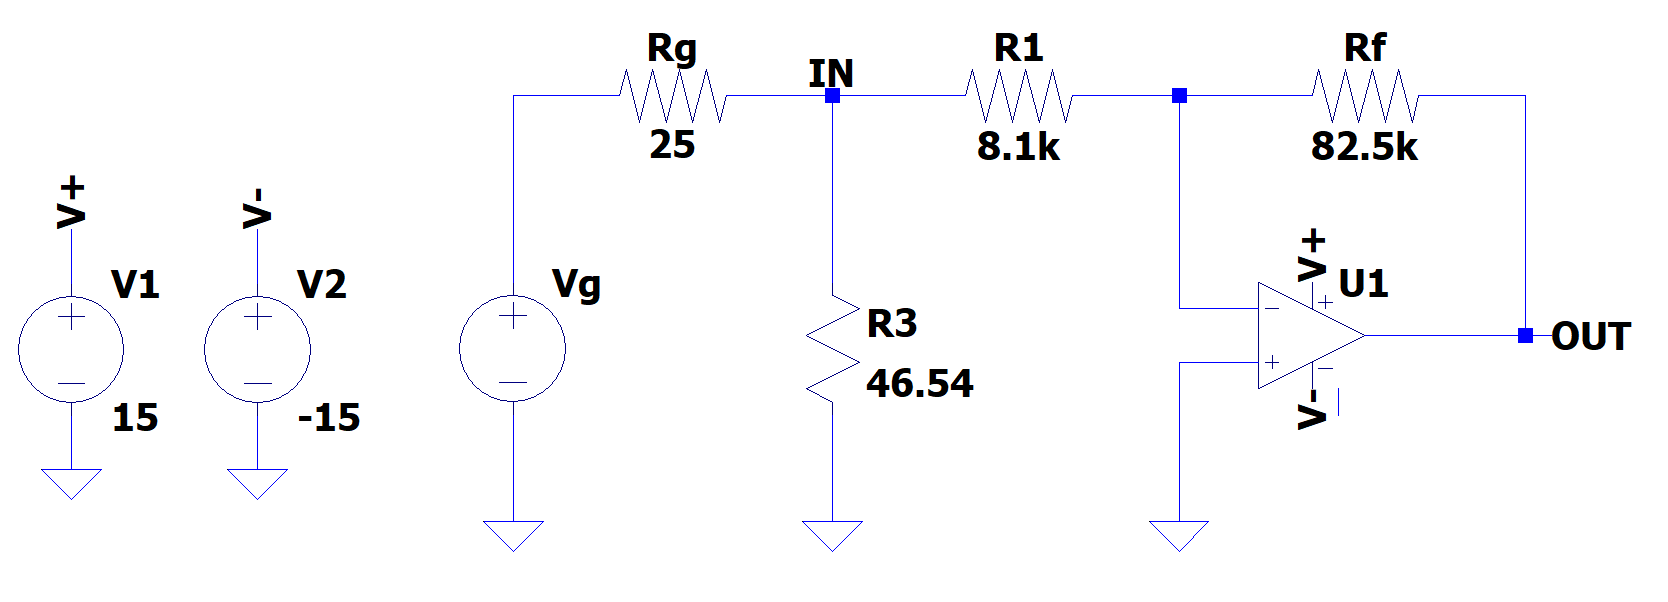
\includegraphics[width=\linewidth]{../Simulations/OpAmp/circuit_image_nosim.png}
	\caption{Rappresentazione a variabili concentrate del circuito assemblato in laboratorio.}
	\label{i:opamp_circuit}
\end{figure}

\noindent Il segnale viene prelevato nei punti \textit{IN} e \textit{OUT} evidenziati nello schema in Figura
\ref{i:opamp_circuit} (e verrà in seguito richiamato rispettivamente come $V_{\text{in}}$ e $V_{\text{out}}$)
utilizzando due sonde con fattore di attenuazione 10X. Nel canale CH1 dell'oscilloscopio viene visualizzato il segnale
in ingresso $V_{\text{in}}$, mentre il segnale in uscita $V_{\text{out}}$ è prelevato dalla sonda collegata al canale
CH2. Per entrambi i canali viene impostata l'attenuazione sonda 10X, in modo da visualizzare nel display il segnale non
attenuato. Il generatore di funzioni viene poi configurato in modalità "50 Ohm", in modo che l'impedenza d'uscita del
generatore sia comparabile con $R_3\approx 50\si{\ohm}$. Così facendo, ci si aspetta di trovare una tensione in ingresso
$V_{\text{in}}$ in accordo con la tensione nominale erogata dal generatore. Si imposta infine il generatore di funzioni
in modo da erogare un segnale di tipo sinusoidale con frequenza $f_{\text{gen}}=1\,\si{k\hertz}$ e di ampiezza
variabile.


\subsection{Acquisizione Misure}
Al fine di verificare la linearità dell'amplificatore operazionale e stimare l'amplificazione del
circuito, si decide di far variare la tensione in ingresso impostando valori crescenti di ampiezza del segnale erogato
dal generatore di funzioni. Per ciascuno di questi valori di tensione si acquisisce la misura di un massimo e di un
minimo sia del segnale $V_{\text{in}}$ sia del segnale $V_{\text{out}}$ sfruttando i cursori orizzontali
dell'oscilloscopio. In questo modo, si ottiene un campione di coppie ($V_{\text{in}}$, $V_{\text{out}}$) che ci si
aspetta segua un andamento lineare. I valori di tensione $V_{\text{gen}}$, $V_{\text{in}}$, $V_{\text{out}}$ e le
relative scale di misura sono riportate in Tabella \ref{}.

\subsection{Simulazioni Spice}
Prima di procedere con l'analisi dati, si decide di simulare la risposta del circuito utilizzando il programma LTSpice.
Il circuito in questione è riportato in Figura \ref{i:opamp_circuit}, tenendo conto però che il generatore è impostato
in modalità "50 Ohm". Si sceglie di effettuare la simulazione considerando due ampiezze in ingresso significative: per
la prima si imposta dal generatore un'ampiezza $V_{\text{gen}}=1\,\si{\volt}$ mentre per la seconda
$V_{\text{gen}}=4\,\si{\volt}$. Questa scelta è dettata dal fatto che l'amplificatore operazionale, essendo una
componente attiva del circuito, non può dare in output una tensiore maggiore di quanta ne riceve in alimentazione
per conservazione dell'energia. 

\begin{figure}[H]
	\centering
	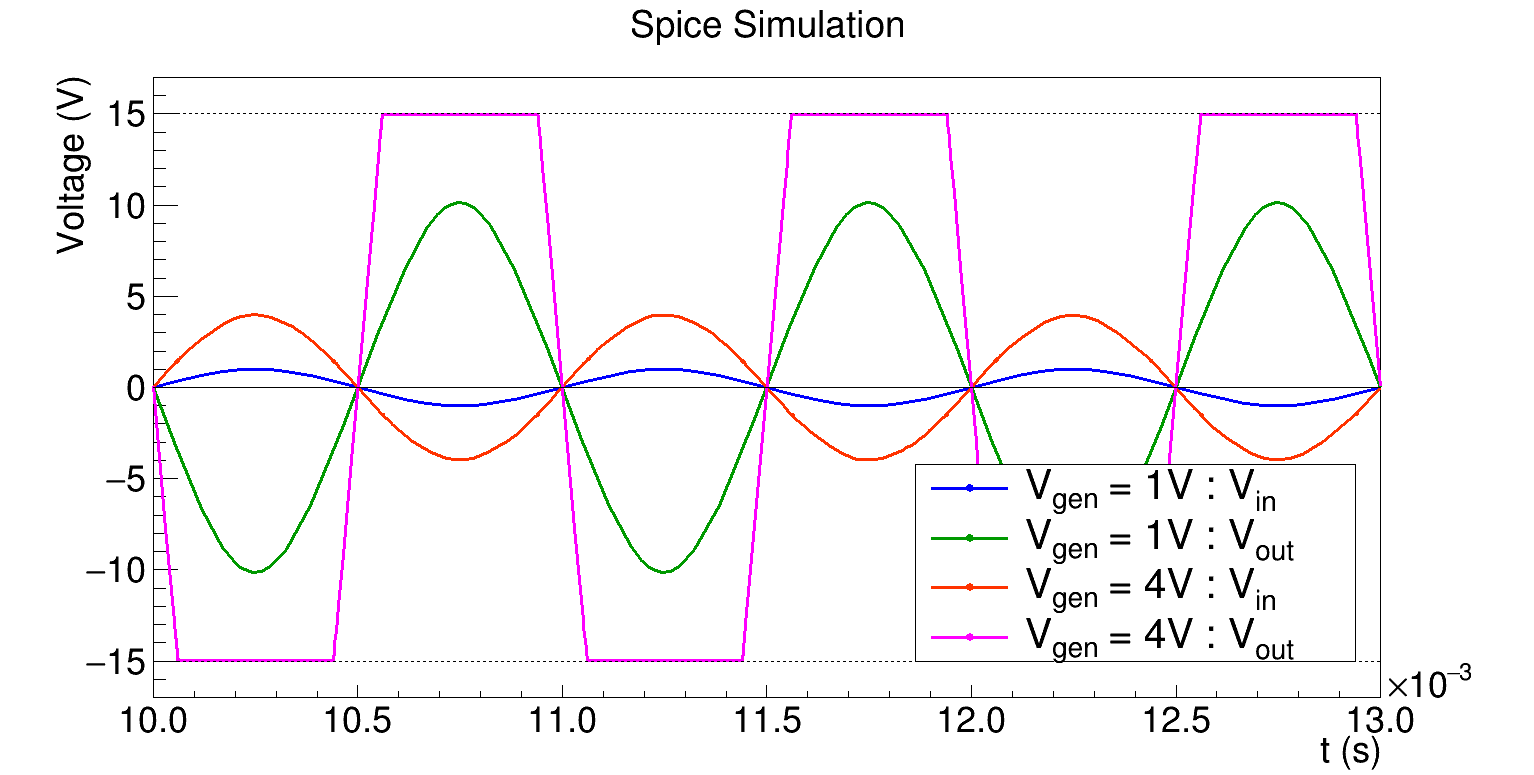
\includegraphics[width=\linewidth]{../Plots/Report_Plots/opamp_spice_1V_4V.png}
	\caption{Simulazione Spice della risposta del circuito ad una tensione sinusoidale in ingresso di frequenza
	$f_{\text{gen}}=1\,\si{k\hertz}$ e ampiezza $V_{\text{gen}}=1\,\si{\volt}$ oppure $V_{\text{gen}}=4\,\si{\volt}$}
	\label{i:opamp_simulation}
\end{figure}

\noindent Dal grafico si evince chiaramente come erogando $V_{\text{gen}}=1\,\si{\volt}$ il segnale viene amplificato
correttamente di circa un fattore 10 mantenendo la forma sinusoidale, mentre erogando $V_{\text{gen}}=4\,\si{\volt}$ il
segnale in uscita presenta i picchi tagliati esattamente a livello delle tensioni di alimentazione fornite
all'operazionale. 

\subsection{Dati e Analisi}
Si riportano in Tabella \ref{} le misure acquisite con l'oscilloscopio, alle quali è stata associata un'incertezza

\begin{equation}
	\sigma_{V} = \sqrt{ (\sigma_{l}\times\text{V/div})^2 + (\sigma_{g}\times\text{measure})^2 }
\end{equation}

\noindent dove $\sigma_{l}=\Delta_{l}/\sqrt{6}$ e $\sigma_{g}=\Delta_{g}/\sqrt{6}$ (assumendo una distribuzione
triangolare) rappresentano l'incertezza di lettura e di guadagno associati all'oscilloscopio, V/div rappresenta la scala
di acquisizione della misura mentre "measure" rappresenta la misura sperimentale stessa.
















\end{document}